\documentclass[%
	corpo=11pt,
    twoside,
    stile=classica,
    oldstyle,
    tipotesi=custom,
    greek,
    evenboxes,
]{toptesi}
%%%%%%%%%%%%%%%%%%%%%%%%%%%%%%%%%%%%%%%%%%%%%%%%%%%%

\usepackage[utf8]{inputenc}
\usepackage[T1]{fontenc}
\usepackage{lmodern}

\usepackage{hyperref}
\hypersetup{%
    pdfpagemode={UseOutlines},
    bookmarksopen,
    pdfstartview={FitH},
    colorlinks,
    linkcolor={blue},
    citecolor={blue},
    urlcolor={blue}
  }

%%%%%%% use PDFLATEX 

\usepackage{lipsum} %to insert random text

\usepackage{geometry} %for the margins
\newcommand\fillin[1][4cm]{\makebox[#1]{\dotfill}} %for the dotted line in the frontispiace

\usepackage{dcolumn}
\newcolumntype{d}{D{.}{.}{-1} } %to vetical align numbers in tables, along the decimal dot

\usepackage{amsmath}

\usepackage{natbib} % for the bibliography
\bibliographystyle{plainnat}

%%%%%%%%%%%%%%%%%%%%
%aggiunti io
\usepackage{graphicx}
\usepackage{subcaption}


%%%%%%% Local definitions
\newtheorem{osservazione}{Osservazione}% Standard LaTeX
\newtheorem{observation}{Observation}% Standard LaTeX


%%%%%%% Custom fonts for title page
\newcommand\customfont[1]{{\usefont{T1}{Poppins-Regular}{m}{n} #1 }}

%%%%%%%%%%%%%%%%%%%%%%%%%%%%%%%%%%%%%%%%%%%%%%%%
%%%%%%%%%%%%%%%%%%%%%%%%%%%%%%%%%%%%%%%%%%%%%%%%



\begin{document}\errorcontextlines=9
%\english

\begin{titlepage}
\newgeometry{left=1cm,right=1cm,top=3cm,bottom=3.5cm}  %specific margins for this page

\begin{center}

{\huge POLITECNICO DI TORINO}\\[1.5cm]
\textbf{Corso di Laurea\\in Matematica per l'Ingegneria}\\[3cm]
%\textbf{Corso di Laurea Magistrale\\in Ingegneria Matematica}\\[3cm]

%{\Large \.}\\[1cm]
%{\Large Tesi di Laurea Magistrale}\\[0.5cm]
\textbf{\LARGE Relazione di Metodi Numerici\\ \,\\per le Equazioni alle Derivate Parziali }\\[2cm]

\includegraphics[width=0.2\textwidth]{./Pictures/logo_polito_2021.jpg}
\vspace{4cm}



Francesco Matteazzi

\vfill

Anno Accademico 2023-2024
\end{center}

\restoregeometry %restor default margins 

\end{titlepage} %the frontispiece

%%%%%%%%%%%%%%%%%%%%%%

\sommario%summary
%Here goes the abstrat of your thesis
La pressione barometrica di Giove viene misurata mediante un metodo originale  messo a punto dai candidati, che si basa sul rilevamento telescopico della pressione.



%%%%%%%%%%%%%%%%%%%%%%%%%%%%%%%%%%%%%%%%%%%%%%%%
%%%%%%%%%%%%%%%%%%%%%%%%%%%%%%%%%%%%%%%%%%%%%%%%

\tablespagetrue\figurespagetrue%to include the list of tables
%and the list of figures - yuo can comment these commands

\indici%table of content
%It automatically generated

%%%%%%%%%%%%%%%%%%%%%%%%%%%%%%%%%%%%%%%%%%%%%%%%
%%%%%%%%%%%%%%%%%%%%%%%%%%%%%%%%%%%%%%%%%%%%%%%%







\mainmatter


%%%%%%%%%%%%%%%%%%%%%%%%%%%%%%%%%%%%%%%%%%%%%%%%%%%%%%%%%%%%%%%
\chapter{Risultati numerici}
In questo capitolo si discutono i risultati numerici ottenuti per alcuni problemi appartenenti alle tipologie descritte nei capitoli precedenti.

\section{Problema di diffusione con condizioni di Dirichlet omogenee}\label{sez-omog}


Si consideri il seguente problema di pura diffusione con condizione di Dirichlet omogenea:
\[
\begin{cases}
-\nu\Delta u = f \text{ in } \Omega \\
u = 0 \text{ su } \partial \Omega\,\,\,;
\end{cases}
\]
 la forzante è \[
 f(x, y) = 32(x(1 - x) + y(1 - y))
 \] e il coefficiente di diffusione $\nu$ è costante e pari a $1.0$. Il dominio è il quadrato  $\Omega = [0, 1] \times [0, 1]$. La soluzione esatta  è \[
 U(x, y) = 16x(1 - x)y(1 - y).
 \]
 

Si calcola la soluzione approssimata su una mesh che viene progressivamente raffinata: il vincolo di area massima per gli elementi della triangolazione cambia ad ogni iterazione, ed è pari a $2^{-4}$,$2^{-5}$,...,$2^{-10}$. La figura \ref{fig:mesh} mostra la triangolazione più raffinata del dominio~$\Omega$.
\begin{figure}[htbp]
  \centering
  %\begin{subfigure}{0.48\textwidth}
    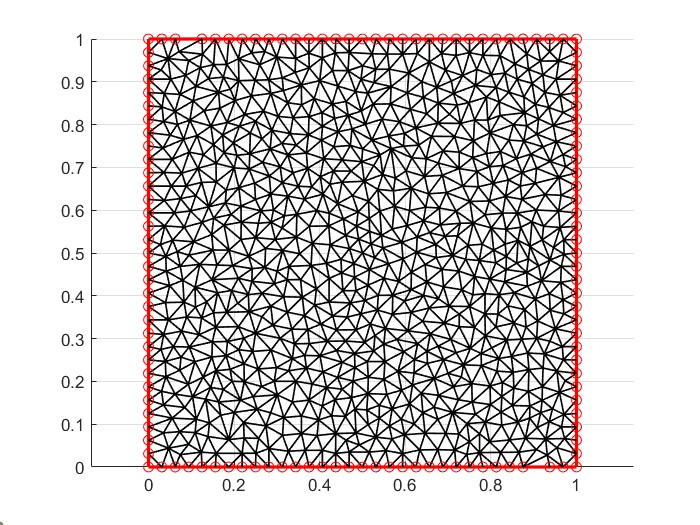
\includegraphics[scale=0.4]{Pictures/triangolazione_2allameno10.jpg}
    \caption{Il dominio $\Omega$, discretizzato con la mesh più fine  (vincolo di area massima pari a $2^{10}$). Qui, $h=0.0697$, $A=7.4855 \cdot 10^{-4}$ e $N_{\text{dof}}=730$}
    \label{fig:mesh}
    \end{figure}


 \subsection{Problema di diffusione  in $P_1$}\label{sez-p1-omog}
Si applica  un metodo di discretizzazione con elementi finiti di Courant, ossia $(T, P_1(T),\\ \{v(\textbf{a}_1)),v(\textbf{a}_2)),v(\textbf{a}_3)\})$.

In figura \ref{fig:soluzione_p1_omog} è riportata la  soluzione approssimata corrispondente alla mesh più fine (fig. \ref{fig:mesh}).


    
\begin{figure}[htbp]
    \centering
    
  %\end{subfigure}
  %\hfill
  %\begin{subfigure}{0.48\textwidth}
    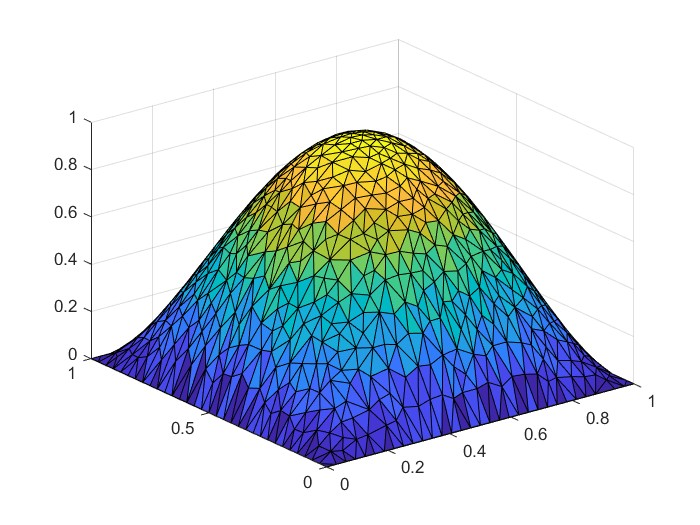
\includegraphics[scale=0.4]{Pictures/grafico_p1_2allameno10_omog.jpg}
    \caption{La soluzione approssimata data dalla mesh più raffinata per il problema di diffusione omogeneo ($P_1$)}
    \label{fig:soluzione_p1_omog}
  %\end{subfigure}
  
\end{figure}


Un'indicazione della correttezza dei risultati è data dal calcolo dell'errore. Esso viene calcolato in norma $L^{\infty}, L^2$ e $H^1$, e in tutti i casi deve risultare coerente con le stime ricavate nella teoria. I parametri secondo cui è valutato sono il passo della triangolazione, l'area massima di un elemento e il numero di gradi di libertà (rispettivamente $h$, $A$ e $N_{dof}$).

Per il caso $P_1$ si ha
\begin{align*}
&\|u - u_h\|_{L^\infty},\,\|u - u_h\|_{L^2} \sim Ch^2 \\
&\;\;\;\;\;\;\;\;\;\;\;\;\;\;\;\;\;\;\;\;\;\;\;\;\;\;\;\;\;\;\;\;\;\;\;\;\;\sim CA^1 \\
&\;\;\;\;\;\;\;\;\;\;\;\;\;\;\;\;\;\;\;\;\;\;\;\;\;\;\;\;\;\;\;\;\;\;\;\;\;\;\sim CN_{\text{dof}}^{-1}
\end{align*}
\begin{align*}
&\|u - u_h\|_{H^1} \sim Ch^1 \\
&\;\;\;\;\;\;\;\;\;\;\;\;\;\;\;\;\;\;\sim CA^{1/2} \\
&\;\;\;\;\;\;\;\;\;\;\;\;\;\;\;\;\;\;\sim CN_{\text{dof}}^{-1/2}
\end{align*}


Nella tabella \ref{tab:stima_errore} si riportano gli esponenti sperimentali ricavati interpolando linearmente il logaritmo del parametro e il logaritmo della norma dell'errore.
\begin{table}[htbp]
  \centering
  \begin{tabular}{|c|c|c|c|}
    \cline{2-4}
    \multicolumn{1}{c|}{} & $h$ & $A$ & $N_{\text{dof}}$ \\
    \hline
    $L^\infty$ & 2.045350  $\approx 2$ & 0.980437 $\approx 1$ & -0.828969 $\approx -1$\\
    \hline
    $L^2$ & 2.115888  $\approx 2$ & 1.020603 $\approx 1$& -0.858987 $\approx -1$\\
    \hline
    $H^1$ & 1.052228  $\approx 1$ & 0.508996 $\approx 0.5$& -0.427547 $\approx -0.5$ \\
    \hline
  \end{tabular}
  \caption{Risultati della stima dell'errore per il problema di diffusione omogeneo ($P_1$). Sono riportati gli ordini di convergenza rispetto a $h$, $A$ e $N_{\text{dof}}$ nelle varie norme}
  \label{tab:stima_errore}
\end{table}

Si analizza anche  il comportamento del numero di condizionamento della matrice di rigidezza. Procedendo come per l'errore, si trova che esso ha ordine $-2.2707\approx-2$ rispetto al passo h, coerentemente con la teoria.

\begin{figure}[htbp]
  \centering
  %\begin{subfigure}{0.48\textwidth}
    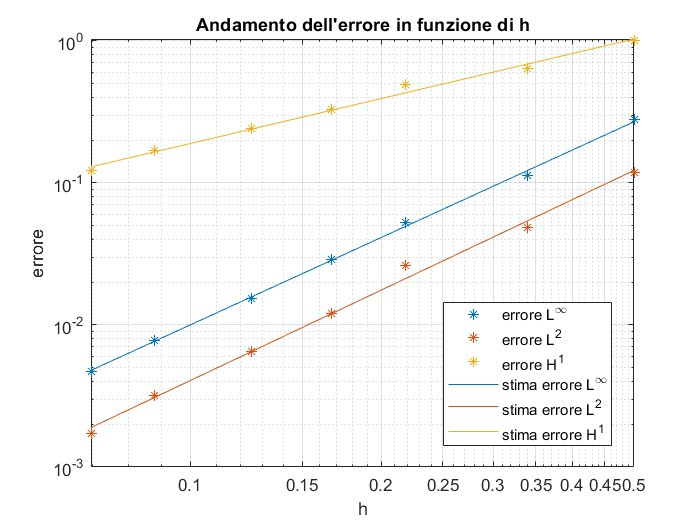
\includegraphics[scale=0.4]{Pictures/errore_h_p1_omog.jpg}
    \caption{Andamento dell'errore in funzione del passo $h$ per il problema di diffusione omogeneo ($P_1$)}
    \label{fig:p1_h}
    \end{figure}
    
    \begin{figure}[htbp]
  \centering
    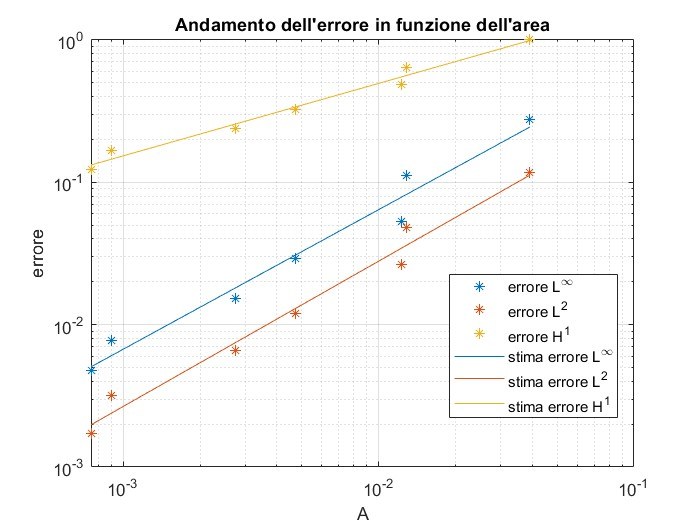
\includegraphics[scale=0.4]{Pictures/errore_area_p1_omog.jpg}
    \caption{Andamento dell'errore in funzione dell'area massima $A$ per il problema di diffusione omogeneo ($P_1$)}
    \label{fig:p1_area}
    \end{figure}
    
    \begin{figure}[htbp]
  \centering
    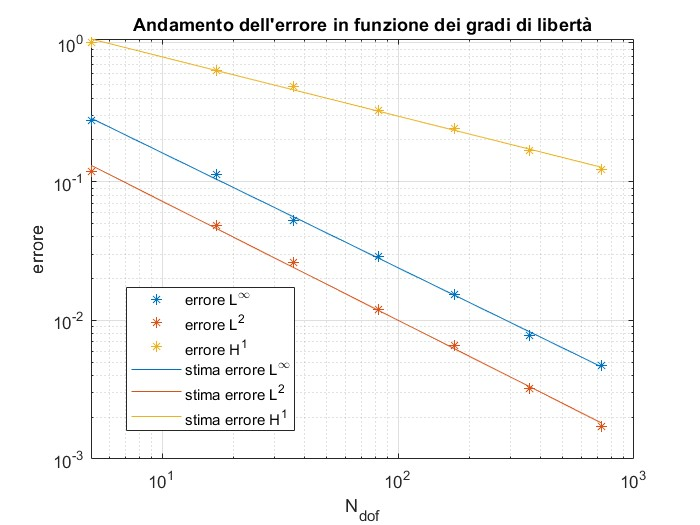
\includegraphics[scale=0.4]{Pictures/errore_gdl_p1_omog.jpg}
    \caption{Andamento dell'errore in funzione del numero dei gradi di libertà $N_{dof}$ per il problema di diffusione omogeneo ($P_1$)}
    \label{fig:p1_gdl}
    \end{figure}

\begin{figure}[htbp]
  \centering
  %\begin{subfigure}{0.48\textwidth}
    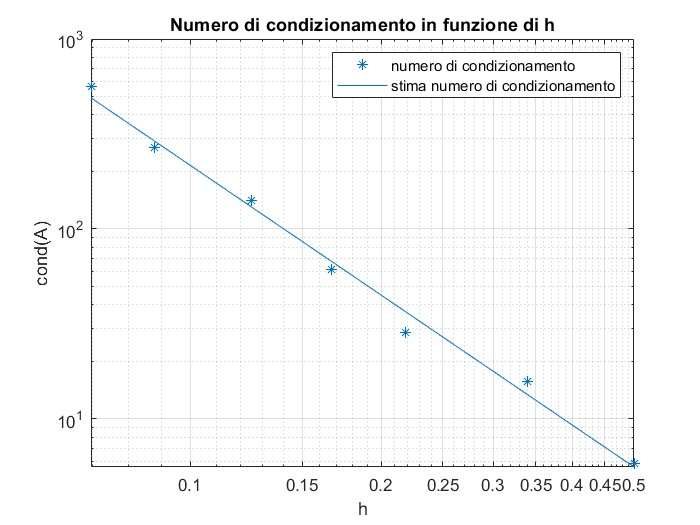
\includegraphics[scale=0.4]{Pictures/condizionamento_p1_omog.jpg}
    \caption{Numero di condizionamento in funzione del passo $h$ per il problema di diffusione omogeneo ($P_1$)}
    \label{fig:p1_cond}
    \end{figure}



%%%%%%%%%%%%%%%%%%%%%%%%%%%%%%%%%
\subsection{Problema di diffusione  in $P_2$}
Si considera il medesimo problema di pura diffusione della sezione \ref{sez-p1-omog}.

Questa volta gli elementi finiti utilizzati sono del tipo $(T, P_2(T), \{v(\textbf{a}_1)),v(\textbf{a}_2)),v(\textbf{a}_3),\\v(\textbf{a}_{1,2})),v(\textbf{a}_{2,3})),v(\textbf{a}_{3,1})\})$, cioè si prende il valore di ?? nei vertici del triangolo e nei punti medi dei tre lati. 

Per $P_2$ valgono le seguenti stime dell'errore: 
\begin{align*}
&\|u - u_h\|_{L^\infty},\,\|u - u_h\|_{L^2} \sim Ch^3 \\
&\;\;\;\;\;\;\;\;\;\;\;\;\;\;\;\;\;\;\;\;\;\;\;\;\;\;\;\;\;\;\;\;\;\;\;\;\;\sim CA^{3/2} \\
&\;\;\;\;\;\;\;\;\;\;\;\;\;\;\;\;\;\;\;\;\;\;\;\;\;\;\;\;\;\;\;\;\;\;\;\;\;\;\sim CN_{\text{dof}}^{-3/2}
\end{align*}
\begin{align*}
&\|u - u_h\|_{H^1} \sim Ch^{3/2} \\
&\;\;\;\;\;\;\;\;\;\;\;\;\;\;\;\;\;\;\sim CA^{1} \\
&\;\;\;\;\;\;\;\;\;\;\;\;\;\;\;\;\;\;\sim CN_{\text{dof}}^{-1}
\end{align*}


\begin{figure}[htbp]
    \centering
    
  %\end{subfigure}
  %\hfill
  %\begin{subfigure}{0.48\textwidth}
    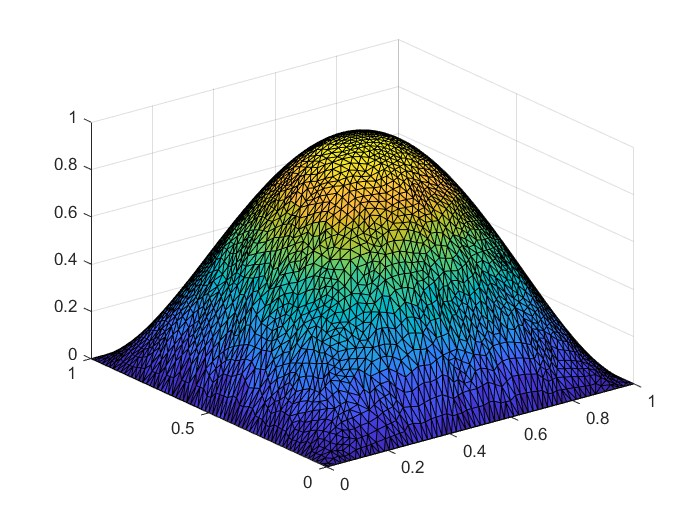
\includegraphics[scale=0.4]{Pictures/grafico-p2-omog.jpg}
    \caption{La soluzione approssimata data dalla mesh più raffinata per il problema di diffusione omogeneo ($P_2$)}
    \label{fig:soluzione_p2_omog}
  %\end{subfigure}
  
\end{figure}



\begin{table}[htbp]
  \centering
  \begin{tabular}{|c|c|c|c|}
    \cline{2-4}
    \multicolumn{1}{c|}{} & $h$ & $A$ & $N_{\text{dof}}$ \\
    \hline
    $L^\infty$ & 3.010940  $\approx 3$ & 1.436332 $\approx 1.5$ & -1.300287 $\approx -1.5$\\
    \hline
    $L^2$ & 3.331096  $\approx 3$ & 1.591100 $\approx 1.5$& -1.441119 $\approx -1.5$\\
    \hline
    $H^1$ & 2.207544  $\approx 2$ & 1.055464 $\approx 1$& -0.95513 $\approx -1$ \\
    \hline
  \end{tabular}
  \caption{Risultati della stima dell'errore per il problema di diffusione omogeneo ($P_2$). Sono riportati gli ordini di convergenza rispetto a $h$, $A$ e $N_{\text{dof}}$ nelle varie norme}
  \label{tab:stima_errore-p2}
\end{table}



\begin{figure}[htbp]
  \centering
  %\begin{subfigure}{0.48\textwidth}
    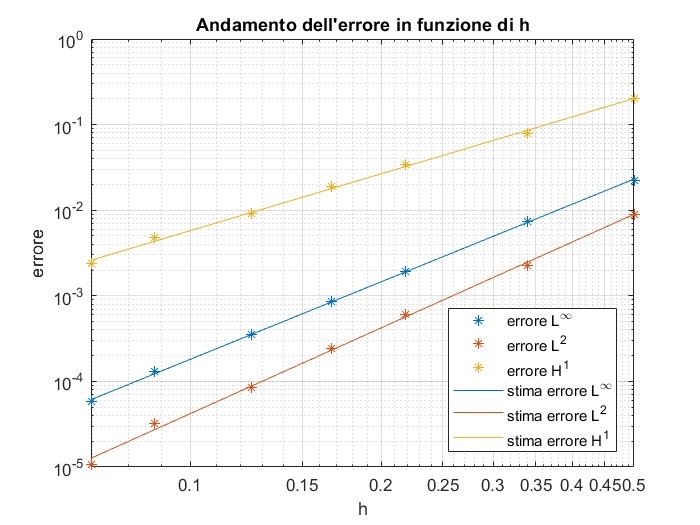
\includegraphics[scale=0.4]{Pictures/errore-p2-h.jpg}
    \caption{Andamento dell'errore in funzione del passo $h$ per il problema di diffusione omogeneo ($P_2$)}
    \label{fig:p2_h}
    \end{figure}
    
    \begin{figure}[htbp]
  \centering
    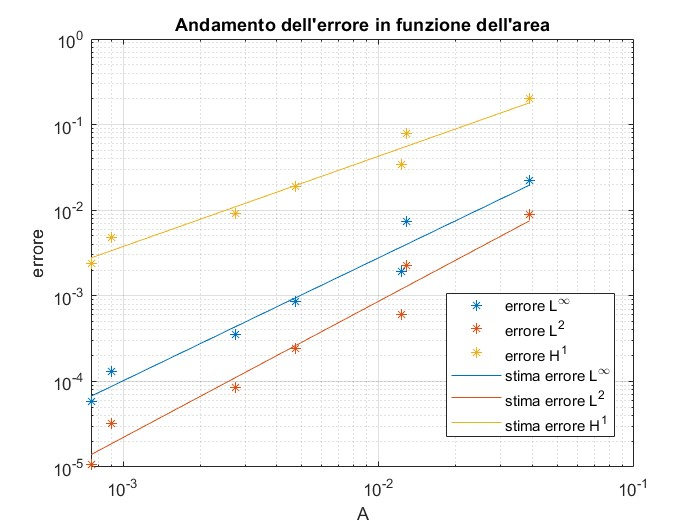
\includegraphics[scale=0.4]{Pictures/errore-p2-area.jpg}
    \caption{Andamento dell'errore in funzione dell'area massima $A$ per il problema di diffusione omogeneo ($P_2$)}
    \label{fig:p2_area}
    \end{figure}
    
    \begin{figure}[htbp]
  \centering
    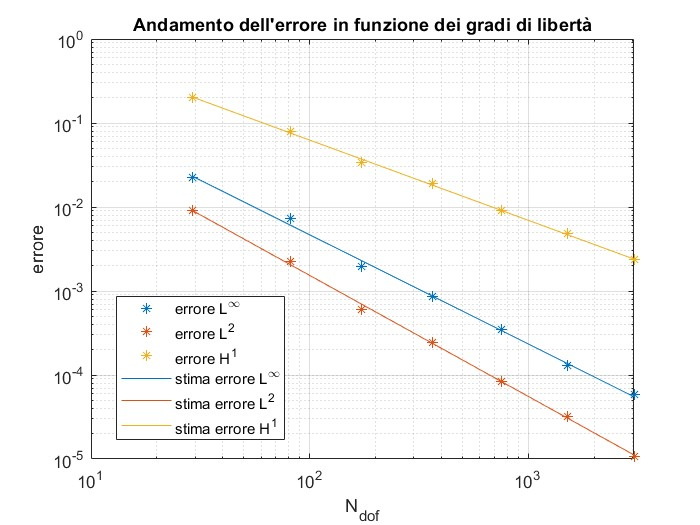
\includegraphics[scale=0.4]{Pictures/errore-p2-gdl.jpg}
    \caption{Andamento dell'errore in funzione del numero dei gradi di libertà $N_{dof}$ per il problema di diffusione omogeneo ($P_2$)}
    \label{fig:p2_gdl}
    \end{figure}

\begin{figure}[htbp]
  \centering
  %\begin{subfigure}{0.48\textwidth}
    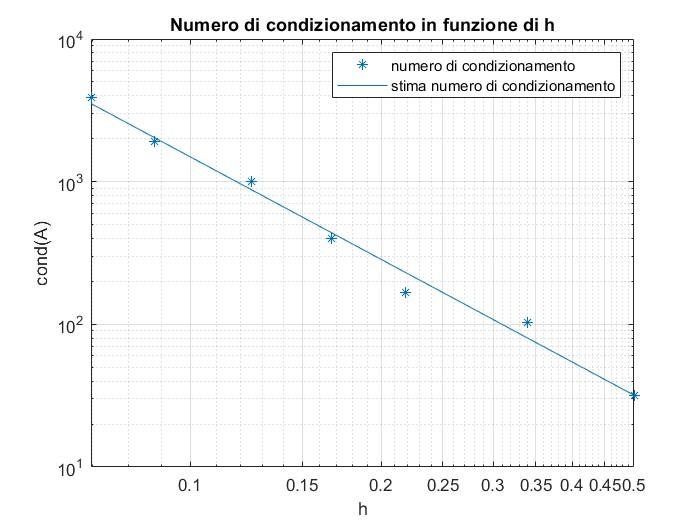
\includegraphics[scale=0.4]{Pictures/condiz-p2.jpg}
    \caption{Numero di condizionamento in funzione del passo $h$ per il problema di diffusione omogeneo ($P_2$)}
    \label{fig:p2_cond}
    \end{figure}


\section[Diffusione-convezione-reazione con condizioni di Dirichlet e  Neumann non omogenee in $P_1$]{Problema di diffusione-convezione-reazione con condizioni di Dirichlet e di Neumann non omogenee in $P_1$}

Si consideri il seguente problema di  diffusione-convezione-reazione con condizioni di Dirichlet e di Neumann non omogenee:
\[
\begin{cases}
-\nu\Delta u + \beta \cdot \nabla u + \sigma u = f \text{ in } \Omega \,\,\,\,\,\,\,\,\,\,\,\,\,\,\,\,\,\,\,\,\,\,\,\Gamma_D\cup\Gamma_N=\partial\Omega, \,\,\,\,\, \Gamma_D\cap\Gamma_N=\emptyset\\
u = g_D \text{ su } \Gamma_D\\
\nu \frac{\partial u}{\partial \hat{\textbf{n}}} = g_N \text{ su } \Gamma_N\,\,\,;\\
\end{cases}
\]
 la forzante è \[
 f(x, y) = (2\pi^2+1)\cos(\pi x)\cos(\pi y) - \pi \sin(\pi x)\cos(\pi y)
 \] e i coefficienti $\nu=\sigma=1.0$, $\beta = (1,\; 0)^T$. Il dominio è sempre il quadrato  $\Omega = [0, 1] \times [0, 1]$, mentre il bordo di Dirichlet è $\Gamma_D = \{1\}\times [0,1]\cup[0,1]\times\{1\}$  e quello di Neumann è $\Gamma_N=\partial\Omega\setminus\Gamma_D$.  La soluzione esatta  è \[
 U(x, y) = \cos(\pi x)\cos(\pi y)\,.
 \]

Valgono i risultati di convergenza dell'errore  visti nella sezione \ref{sez-p1-omog}.

\begin{figure}[htbp]
    \centering
    
  %\end{subfigure}
  %\hfill
  %\begin{subfigure}{0.48\textwidth}
    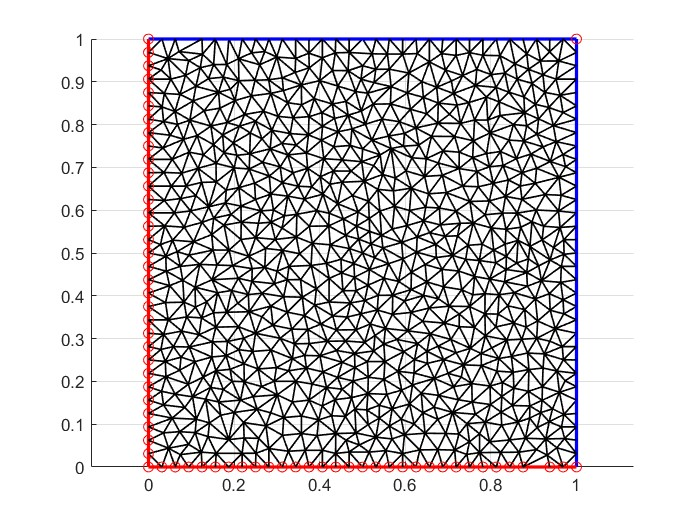
\includegraphics[scale=0.4]{Pictures/mesh_p1_neumann.jpg}
    \caption{Il dominio $\Omega$, discretizzato con la mesh più fine  (vincolo di area massima pari a $2^{10}$). La porzione del bordo evidenziata in blu ha condizione di Neumann, quella in rosso ha condizione di Dirichlet}
    \label{fig:mesh_neumann}
  %\end{subfigure}
  
\end{figure}


\begin{figure}[htbp]
    \centering
    
  %\end{subfigure}
  %\hfill
  %\begin{subfigure}{0.48\textwidth}
    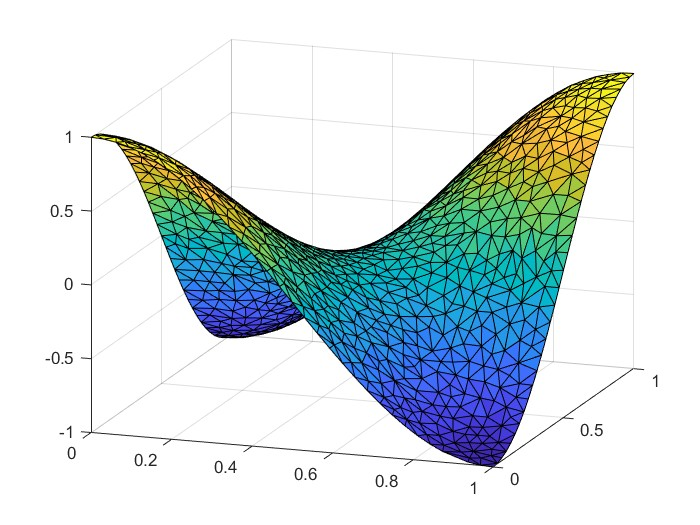
\includegraphics[scale=0.4]{Pictures/grafico_funzinv.jpg}
    \caption{La soluzione approssimata data dalla mesh più raffinata per il problema di diffusione-convezione-reazione}
    \label{fig:soluzione_neumann}
  %\end{subfigure}
  
\end{figure}



\begin{table}[htbp]
  \centering
  \begin{tabular}{|c|c|c|c|}
    \cline{2-4}
    \multicolumn{1}{c|}{} & $h$ & $A$ & $N_{\text{dof}}$ \\
    \hline
    $L^\infty$ & 1.917338  $\approx 2$ & 0.914744 $\approx 1$ & -0.862855 $\approx -1$\\
    \hline
    $L^2$ & 2.154033  $\approx 2$ & 1.031071 $\approx 1$& -0.971995 $\approx -1$\\
    \hline
    $H^1$ & 1.105088  $\approx 1$ & 0.532438 $\approx 0.5$& -0.498622 $\approx -0.5$ \\
    \hline
  \end{tabular}
  \caption{Risultati della stima dell'errore per il problema di diffusione-convezione-reazione. Sono riportati gli ordini di convergenza rispetto a $h$, $A$ e $N_{\text{dof}}$ nelle varie norme}
  \label{tab:stima_errore-neumann}
\end{table}




\begin{figure}[htbp]
  \centering
  %\begin{subfigure}{0.48\textwidth}
    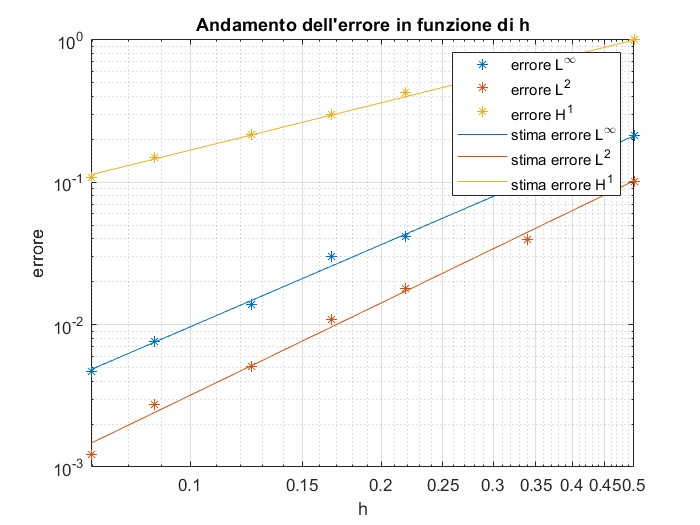
\includegraphics[scale=0.4]{Pictures/errore-neumannfunzinv-h.jpg}
    \caption{Andamento dell'errore in funzione del passo $h$ per il problema di diffusione-convezione-reazione}
    \label{fig:neumann_h}
    \end{figure}
    
    \begin{figure}[htbp]
  \centering
    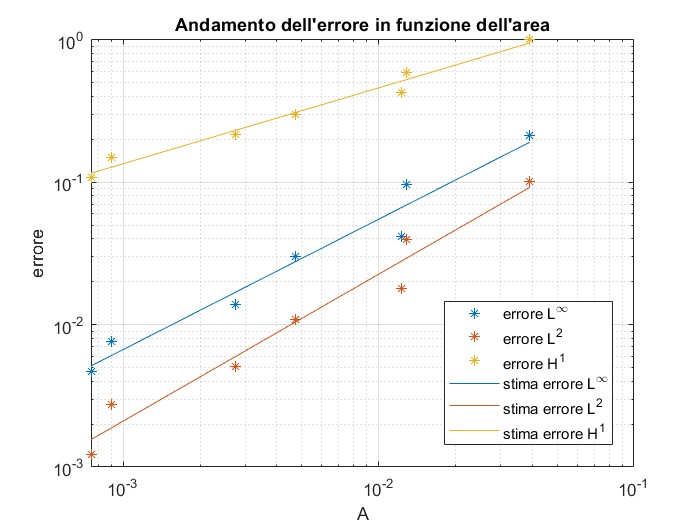
\includegraphics[scale=0.4]{Pictures/errore-neumann-funzinv-area.jpg}
    \caption{Andamento dell'errore in funzione dell'area massima $A$ per il problema di diffusione-convezione-reazione}
    \label{fig:neumann_area}
    \end{figure}
    
    \begin{figure}[htbp]
  \centering
    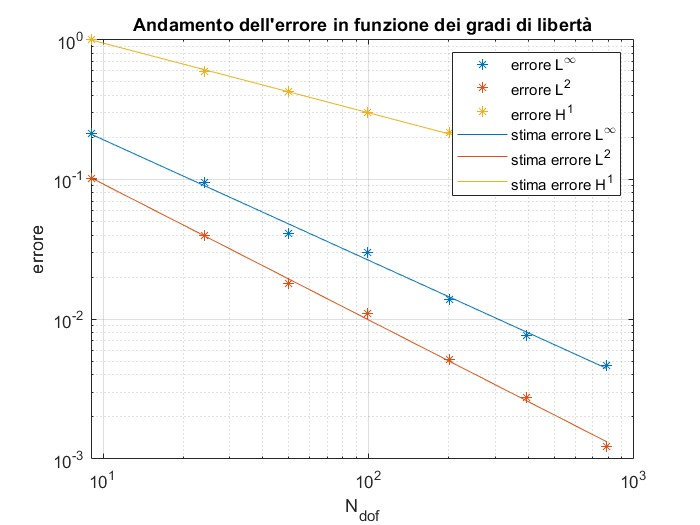
\includegraphics[scale=0.4]{Pictures/errore-neumannfunzinv-gdl.jpg}
    \caption{Andamento dell'errore in funzione del numero dei gradi di libertà $N_{dof}$ per il problema di diffusione-convezione-reazione}
    \label{fig:neumann_gdl}
    \end{figure}

\begin{figure}[htbp]
  \centering
  %\begin{subfigure}{0.48\textwidth}
    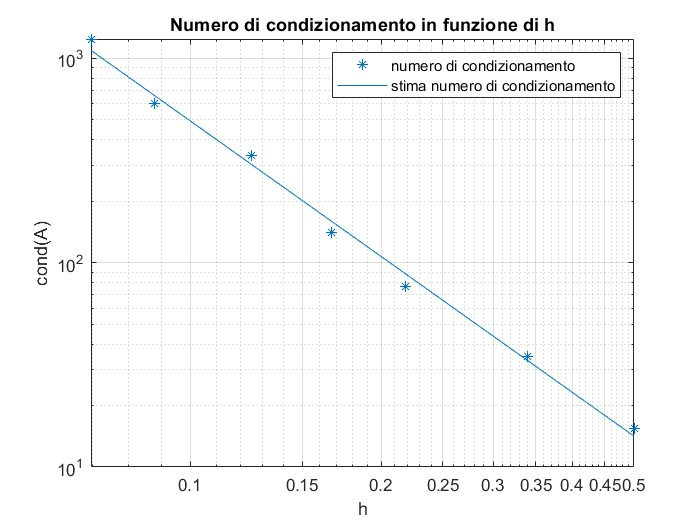
\includegraphics[scale=0.4]{Pictures/condiz-neumannfunzinv.jpg}
    \caption{Numero di condizionamento in funzione del passo $h$ per il problema di diffusione-convezione-reazione}
    \label{fig:neumann_cond}
    \end{figure}

ordine numero condiz: -2.206987

%%%%%%%%%%%%%%%%%%%%%%%%%%%%%%%%%%%%%%%%%%%%%%%%

%\bibliography{references}



\end{document}

